\documentclass[11pt]{article}

\usepackage{amssymb,amsmath}
\usepackage{times,psfrag,epsf,epsfig,graphics,graphicx,caption}
\usepackage{enumitem,fontawesome}
\usepackage{algorithm}
\usepackage{algorithmic}



\begin{document}
\date{}

\title{PHSX 343: Assignment 13}

\author{William Jardee}

\maketitle

\section*{Problem 1}
    \[v_x = \frac{E}{B}\]
    Checking to see if this is relativistic first: 
    \[K=\frac{1}{2}m_ev^2 \rightarrow v = \sqrt{\frac{2K}{m_e}} = 0.44c\]
    So this is definitely relativistic
    \[\frac{u}{c}=\frac{Pc}{E}=\frac{\sqrt{E^2 - (m_ec^2)^2}}{m_ec^2+k} = 0.413c\]
    Now using this value in the first equation:
    \[B = \frac{E}{v_x} = 0.00162T = \boxed{1.6 mT}\]

\section*{Problem 2}
    In order to solve this one I followed example 4.3 in the book pretty closely and wrote a quick python script to make my life a lot easier.\\
    \begin{center}
     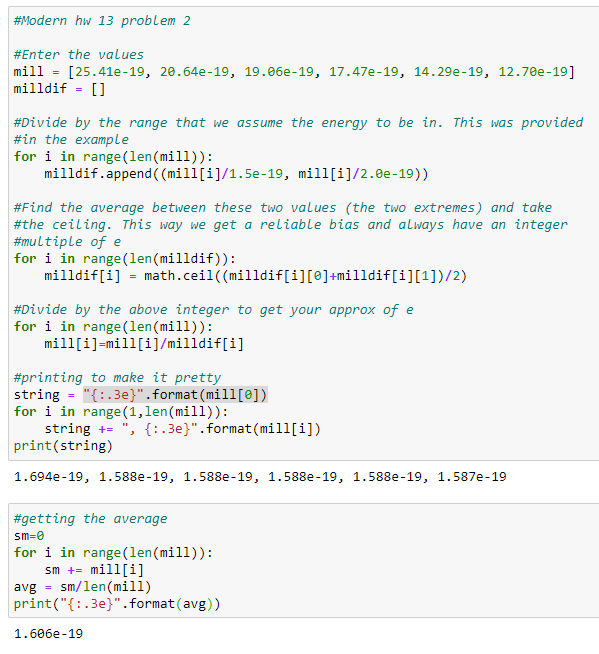
\includegraphics[width = 400]{Homework13/problem 2.PNG}
    \end{center}
    All the math is laid out there, but for the answer, what was wanted was a little confusing. What I have settled on is to give the format of both ways we understood the question. If the question just wanted us to pull out the largest value out of the array, the charge is $e=1.694\times 10^{-19} C$. In the example they took the average, and I can see the question asking that in a very odd way, so the average is $e=1.606 \times 10^{-19}C$.



\section*{Problem 3}
    Pulling the equation from class:
    \[d_{min} = \frac{kq_\alpha Q}{K_\alpha}\]
    \[K_\alpha = \frac{kq_\alpha Q}{r_{al}} = \frac{8.988 \time 10^9 \cdot 2e \cdot 13e}{3.6 \times 10^{-15}} = 1.666 \times 10^{-12} J = 10.4 MeV\]
    Now to check that this resulting equation isn't relativistic:\\
    \[m = 3.727 \frac{GeV}{c^2}\]
    \[\frac{u}{c} = \frac{Pc}{mc^2} = \frac{\sqrt{(mc^2 + K)^2 - (mc^2)^2}}{mc^2 + K} = 0.0745\]
    Since $0.0745 < 0.1$ the speed is not relativistic.
    
\section*{Problem 4}    
    \[\frac{\Delta n}{\Delta t} = \Big(\frac{\frac{dn_{inc}}{dt}NA}{R^2}\Big)\Big(\frac{kZe^2}{2K}\Big)^2\frac{1}{sin^4(\frac{\phi}{2})}\]
    Now, using all the values:\\
    $A = 0.5\times 10^{-4} m$, $z=47$, $\frac{dn_{inc}}{dt} = \frac{1\times 10^{-9}}{2e}$, $R = 0.1 m$, $e=1.602 \times 10^{-19} C$, $k = 8.988\times 10^9$., $K = 9.613 \times 10^{-13} J$, $D = 1 \times 10^{-6} m$.
    To get N, we can just use $\frac{atoms}{vol} = \frac{\rho N_a}{M}$. Then if we multiply by the height, we get the number of atoms in that resulting cut-out. \\
    With values: $M = 107.8682\frac{g}{mol}$, $\rho = 10.49 \times 10^6 \frac{g}{m^3}$, $N_a = 6.022 \times 10^{23} \frac{atoms}{mol}$
    \[N = \frac{\rho DN_a}{M} = 5.856 \times 10^{22}\]
    Now, plugging in all these values into an online calculator:\\
    $\theta = 60^o$:
    \[\frac{\Delta n}{\Delta t} = 460 \frac{atoms}{s}\]
    $\theta = 120^o$:
    \[\frac{\Delta n}{\Delta t} = 52 \frac{atoms}{s}\]






    \begin{flushright}
\includegraphics[width = \linewidth]{Homework13/photo1.jpg}
    \end{flushright}
    
\end{document}
